\chapter{浅表淋巴结肿大}

淋巴结广泛分布于全身,不但是免疫器官,也是造血器官,是机体接受抗原刺激产生免疫应答的场所。其主要功能是对细菌、异物的吞噬产生免疫球蛋白和淋巴因子及参与髓外造血。正常淋巴结多呈卵圆形或豆形、质地软、光滑、无压痛、可以滑动,与毗邻组织无粘连,直径一般不超过0.5cm,除在颌下、腋窝、腹股沟可触及1~3个淋巴结以外,一般不容易触及。如在枕后、耳周、滑车上、锁骨上等部位触及淋巴结则属异常。浅表淋巴结按组群分布,每一个部位的淋巴结属一组,一个组群的淋巴结收集一定区域的淋巴液,局部的炎症或肿瘤转移,首先引起相应区域的淋巴结肿大。当一组淋巴结肿大时,称为局限性淋巴结肿大,若两组以上的淋巴结肿大则称为全身性淋巴结肿大。按淋巴结肿大的发生机制可将淋巴结肿大分类为:①免疫应答所致的淋巴结肿大,这是由全身或局部感染,机体发生免疫应答反应而导致淋巴结肿大。②淋巴结感染所致的淋巴结肿大。③原发于淋巴结的肿瘤或肿瘤的淋巴结转移。④原因不明的疾病所致淋巴结肿大。表\ref{tab32-1}列举了常见的导致淋巴结肿大的病因。

浅表淋巴结肿大的诊断思路和检查步骤:淋巴结肿大往往是全身性疾病的局部表现,所以必须通过详尽询问病史,全面准确的体格检查,除常规实验室检查外,针对根据病史、体检、常规实验室检查综合分析后疑及的诊断有选择地做相应的特殊检查,必要时行淋巴结穿刺、印片或整个淋巴结切除病理活检,或其他组织活检,或淋巴系统造影等,综合分析,以便尽快确定诊断。

\section{【病史】}

流行病史对急性传染病所致的淋巴结肿大往往能提供重要的诊断线索。口腔和咽喉感染常引起颌下淋巴结肿痛。下肢和外生殖器感染,常导致腹股沟淋巴结肿痛。胸锁乳突肌后淋巴结肿大时,应询问有无鼻塞、鼻出血,并作鼻咽部检查以排除或证实鼻咽癌的存在等。对于有野外活动、有皮肤焦痂伴焦痂附近淋巴结肿痛者,应做外-斐反应或补体结合试验,以证实恙虫病的诊断。性病性肉芽肿引起的淋巴结肿大,往往能询问到冶游史(或配偶冶游史)。进行性无痛性淋巴结明显肿大,往往提示恶性淋巴瘤。服用苯妥英后出现淋巴结肿大应考虑苯妥英所致,停药后淋巴结消退可以验证这一推断。毒蛇咬伤常引起相应部位淋巴结肿大。

\section{【体征】}

\subsection{(一)部位}

\subsubsection{1.全身性淋巴结肿大}

可见于某些全身性感染(如结核病、传染性单核细胞增多症等)、白血病、恶性淋巴瘤、过敏性疾病、艾滋病、结缔组织病等。

\subsubsection{2.局限性淋巴结肿大}

常由于局限性感染引起,但也可见于全身性疾病,如恶性淋巴瘤、恶性肿瘤的转移、全身性感染性疾病如弓形虫病等。如发现女性患者单侧腋窝淋巴结明显肿大时,应仔细检查同侧乳房有无乳腺癌的体征,应考虑乳腺癌、黑色素癌转移或淋巴细胞为主型的霍奇金淋巴瘤。枕部淋巴结肿大伴斑丘疹,则是风疹(或弓形虫病)的典型表现。锁骨上淋巴结肿大应考虑淋巴结转移癌(左侧锁骨上淋巴结转移多见于胃癌,右侧可见于支气管癌)。双侧颈部淋巴结肿痛最常见的局部感染是病毒、支原体、链球菌、金葡菌或表葡菌所致的咽炎或扁桃体炎,单侧颈部淋巴结肿痛通常是化脓性扁桃体炎、腮腺炎或牙周脓肿的结果。

\begin{table}[htbp]
\centering
\caption{淋巴结肿大的分类}
\label{tab32-1}
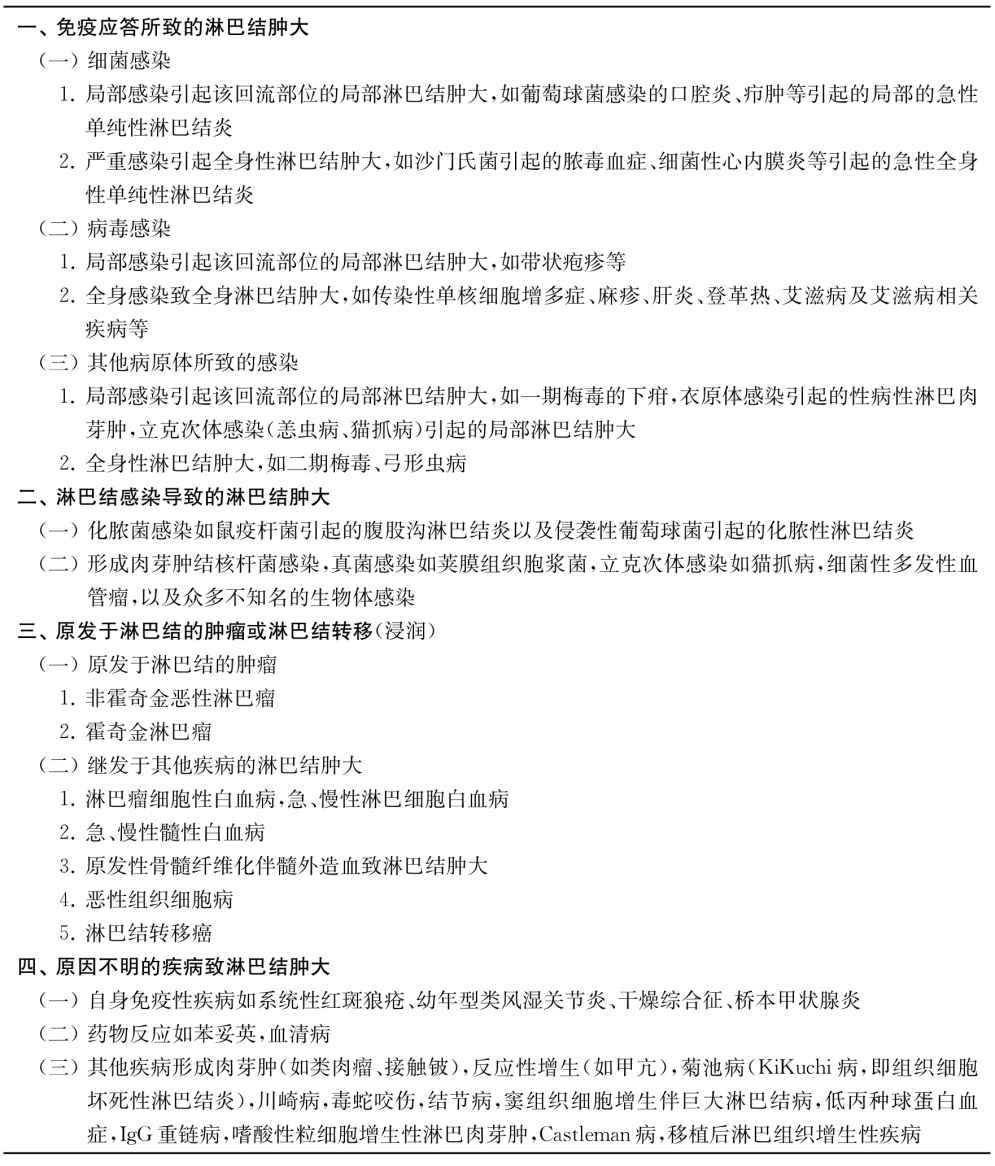
\includegraphics[width=5.86458in,height=6.875in]{./images/Image00161.jpg}
\end{table}

\subsection{(二)数量和大小}

儿童颈部如串珠状的多个淋巴结肿大应警惕淋巴结结核的可能。由于小儿和青少年更易受到新抗原的刺激,致使小儿和青少年淋巴结/体重的比值比成年人大,所以同样的肿大在成年人中有意义而在小儿和青少年中则可能无意义。局限性淋巴结明显肿大可见于癌症转移、恶性淋巴瘤等。全身性淋巴结明显肿大可见于白血病、恶性淋巴瘤、Castleman病等。

\subsection{(三)质地}

感染引致的肿大淋巴结通常质地软,且通常具有表面粗糙的特点(如在一些腔道内形成肿块,则应注意一些特殊的感染,如曲菌病、结核病、放线菌病。所有感染所致的淋巴结肿大通常都会随感染的消除而缩小)。免疫因素所致的肿大淋巴结质地也常常是软的。淋巴结转移癌通常质地坚实,无痛、逐渐增大,表面皮肤正常,常多个互相粘连并与基底黏着,移动性差。淋巴瘤所致的淋巴结肿大则通常质韧实有弹性,触之如橡胶,大多数情况下移动性好,但少数淋巴结巨大者或淋巴结互相融合者则移动性差,但质地坚硬而有弹性。值得注意的是,Ki-1(+)的间变性大细胞性非霍奇金恶性淋巴瘤有类似感染性淋巴结炎的征象。

\subsection{(四)压痛}

颌下、腹股沟淋巴结正常可被触及,但无压痛。如这些淋巴结有自发性疼痛或(及)压痛,提示为病理性。大多数情况下,有压痛或自发痛的通常为炎症性(感染、药热、血清病)。但转移癌或恶性淋巴瘤增大过快时,也可有自发痛和压痛。局限性淋巴结肿痛,常提示其收纳范围组织或器官有活动性感染灶。腹股沟淋巴结剧烈肿痛(痛性下疳)见于软性下疳链杆菌感染,淋巴结易于化脓溃破形成穿凿状溃疡(溃疡基底脓液涂片可找到软性下疳链杆菌)。猫抓病受累的淋巴结肿大为局限性、疼痛也较明显,也可化脓且偶有形成瘘管者。

\subsection{(五)移动性}

肿大的淋巴结互相粘连,或与基底组织粘连,可见于晚期恶性淋巴瘤和结核性淋巴结炎。癌细胞浸润也可导致淋巴结与基底组织粘连而移动性差。

\subsection{(六)波动感和瘘管}

淋巴结有波动感提示淋巴结化脓、坏死软化。结核性淋巴结炎、放线菌病或性病性腹股沟淋巴肉芽肿可引起淋巴结破溃形成瘘管,瘘管愈合后遗留瘢痕;而淋巴结转移癌和恶性淋巴瘤的淋巴结一般不溃破形成瘢痕。

\section{【实验室检查与器械检查】}

\subsection{(一)血常规检查}

外周血发现原始及幼稚细胞提示白血病;白细胞及中性粒细胞增高提示细菌感染;白细胞增多(或正常)伴异形淋巴细胞>10\%提示传染性单核细胞增多症。

\subsection{(二)血沉}

明显增快提示活动性结核、风湿性疾病活动期、淋巴瘤、白血病等。

\subsection{(三)骨髓涂片(包括活检)检查}

可确诊白血病、淋巴瘤(当淋巴瘤细胞侵犯骨髓时)、黑热病(当发现杜氏利什曼原虫,可确诊黑热病)。

\subsection{(四)病原体检查}

如急性全身性感染性疾病血培养、淋巴结瘘管分泌物找病原体、性病性肉芽肿时做分泌物衣原体分离培养或(及)Frei试验。

\subsection{(五)免疫学检查}

如疑及恙虫病时做外-斐反应。疑及弓形虫病时可查弓形虫抗体。疑及自身免疫性疾病时可作相应抗体检查。

\subsection{(六)特殊器械检查}

胸部X线检查可发现肺部与纵隔病变。B超、CT、MRI或PET-CT检查更有利于发现纵隔、腹膜后淋巴结肿大,但未能代替病理活检。PET-CT能同时提供功能和解剖信息,且能够发现全身隐匿病病灶,提供合适的活检部位。

\subsection{(七)病理检查}

淋巴结穿刺、印片及活体组织检查各有其优缺点,可根据具体情况选择进行。由于穿刺吸取组织细胞较少,涂片厚薄不均致阳性物质定位不清而出现假阳性,更不能根据需要连续切片,故有条件者尽可能行淋巴结活检,但应注意淋巴结活检有时可呈阴性结果,当高度怀疑为某一疾病时应反复检查,有时需多次活检才能确诊。如有多个淋巴结肿大原则上应选取最大的淋巴结作活检,并整个切下。如多部位淋巴结肿大,优先考虑作锁骨上淋巴结活检,其次是颈后、腋下,最后才考虑腹股沟淋巴结。

\subsection{(八)淋巴系统造影}

用X线淋巴系统造影可了解淋巴结的改变,帮助鉴别诊断。例如,炎症性淋巴结肿大,其边缘及内部结构正常;转移癌侵犯的淋巴结则边缘不规则如虫蚀样,结内有充盈缺损,如果淋巴结完全被癌组织所占据则无此征象,但有继发性淋巴管阻塞。恶性淋巴瘤则淋巴结数目和大小均增加,边缘光滑,但内部结构被破坏成泡沫状,霍奇金淋巴瘤淋巴结中心还可见充盈缺损。超声造影借助造影剂增强后散射回声,能明显提高超声诊断的分辨力、敏感性和特异性。

淋巴结肿大在临床上可分为急性和慢性两大类,病因很多(表\ref{tab32-2})。现按表中顺序讨论如下。

\begin{table}[htbp]
\centering
\caption{淋巴结肿大的病因}
\label{tab32-2}
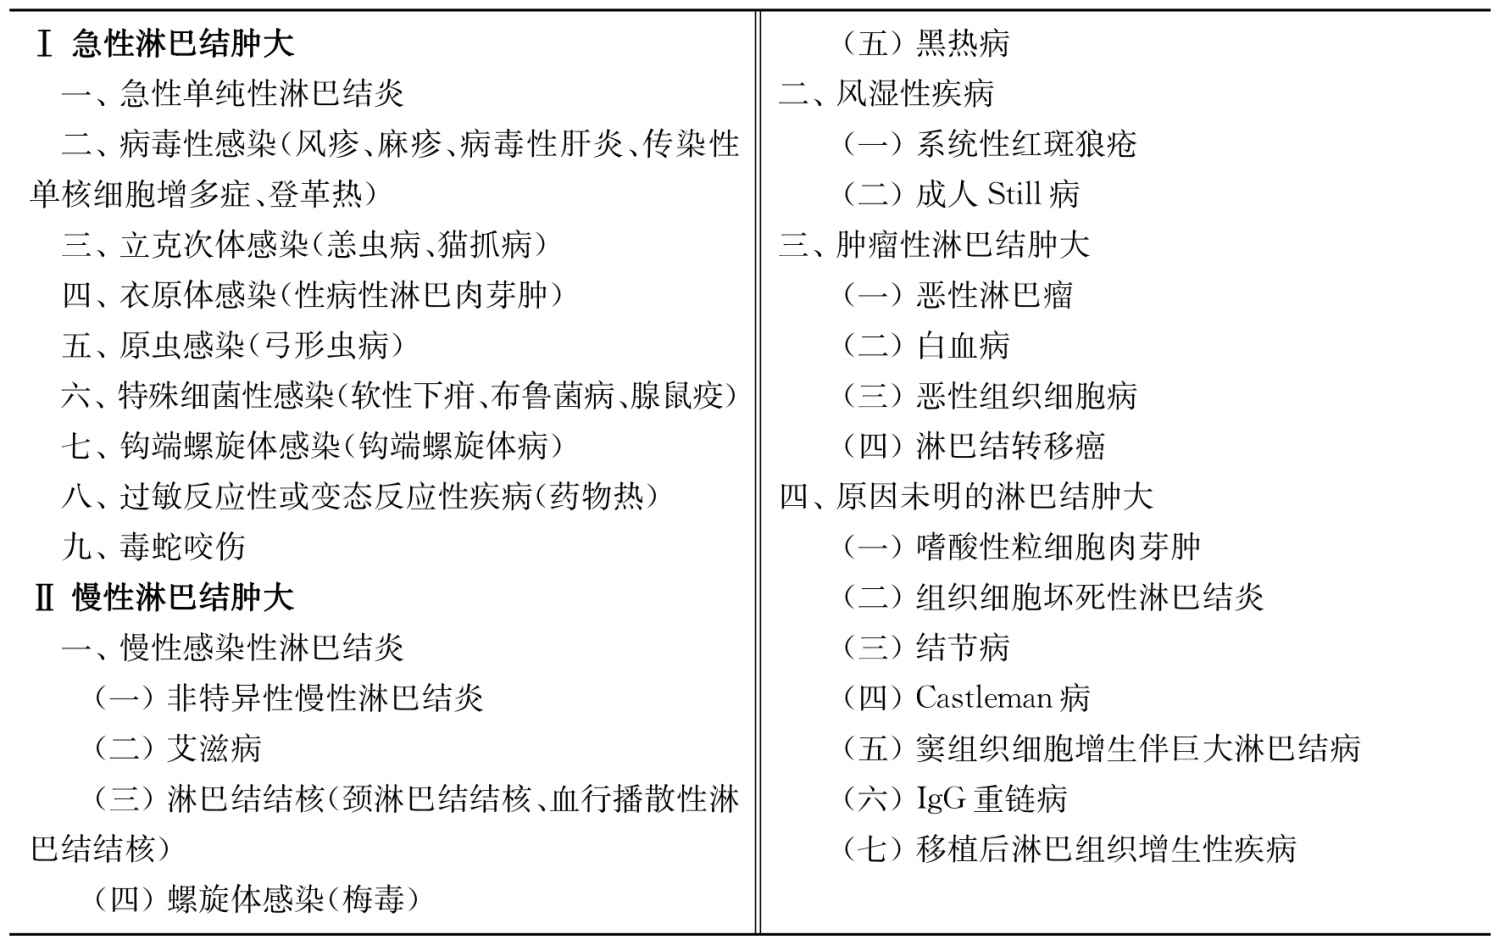
\includegraphics[width=5.89583in,height=3.72917in]{./images/Image00162.jpg}
\end{table}

\protect\hypertarget{text00253.html}{}{}

\section{110 急性淋巴结肿大}

\subsection{一、急性单纯性淋巴结炎}

一般局部都有明显的红、肿、热、痛,常为肿痛性局限性淋巴结肿大,皮肤可潮红,质地软至中等硬度,有自发痛和压痛,表面光滑,无粘连,肿大到一定程度即停止,与原发病灶部位有关,因此,应寻找局部淋巴结收纳范围的原发病灶。如头皮感染可引起枕部和耳后淋巴结炎,口腔和咽部急性炎症可引起颌下淋巴结炎。往往白细胞升高,中性粒细胞增多。

\subsection{二、病毒性感染}

常见者有风疹、麻疹、传染性单核细胞增多症、病毒性肝炎、登革热等。风疹可伴有轻度淋巴结肿大,其特征是位于乳突内侧的耳后、枕骨下和颈后淋巴结肿大,有压痛,与皮疹同时出现,流行病学资料,发热,向心性皮疹(掌心和足底无皮疹),风疹抗体阳性。麻疹特征是发热、上呼吸道卡他症状,起病第2~3天(出疹前)在双侧近臼齿颊黏膜处出现麻疹黏膜斑对出疹早期诊断极有帮助,病情进展极期出疹,疹退后留下色素斑伴糠麸样脱屑。病毒性肝炎可伴淋巴结肿大,但各型病毒性肝炎均可通过常规检测其病毒抗原或抗体的标志和肝功能等而获确诊。传染性单核细胞增多症可引起全身性淋巴结肿痛,尤以颈部为多见,发热、咽痛、血象淋巴细胞增多,异形淋巴细胞>10\%,骨髓象除异形淋巴细胞增多(比外周血比例低)外无特殊改变,嗜异性凝集试验及EB病毒IgM抗体阳性可确定诊断。登革热全身淋巴结可轻度肿大,鞍形热、头痛,眼眶痛,关节肌肉剧痛,热后两天出现皮疹、白细胞和血小板减少,出血倾向,病毒分离和补体结合试验可确诊。

\subsection{三、立克次体感染}

\subsubsection{(一)恙虫病}

可引起局限性(焦痂附近)或全身性淋巴结肿大,肿大的淋巴结皆有自发痛与压痛,常伴发热、头痛、疲倦、食欲不振、咳嗽等表现,肝脾大、肺部少量湿性啰音、肝功能异常较为常见。焦痂为本病的特征性体征,有极其重要的诊断意义。局部淋巴结肿痛常提示焦痂所在的部位。疫区野外活动史,外-斐反应阳性,补体结合试验、间接免疫荧光试验或固相放射免疫试验可协助确诊。巢式聚合酶链反应特异性和敏感性较高。

\subsubsection{(二)猫抓病}

有与猫狗等宠物接触并被猫狗等抓、咬伤史,典型的表现是在被猫抓伤或咬伤的部位出现类似昆虫咬伤的小皮损,3~10天后在抓痕处形成圆形、棕红色、无痛的丘疹,脓疮、1~2周后出现1枚或1枚以上引流区域的淋巴结肿大,受累淋巴结以肘部、腋部、颈部常见,多数有触痛,少数可化脓触之有波动感,偶可引起瘘管,部分患者有发热、全身不适及肝脾大等,特异性抗原皮内试验阳性可验证诊断。主要病理特征是淋巴结微脓肿性肉芽肿性炎,Warthin-starry银染色可见汉氏巴尔通体,新型抗汉赛巴尔通体单克隆抗体染色法检出汉赛巴尔通体的阳性率显著高。

\subsection{四、衣原体感染}

性病性淋巴肉芽肿(第四性病):患者因感染性病性淋巴肉芽肿衣原体引起腹股沟淋巴结肿大。病初首先在外生殖器上出现无痛性溃疡或丘疹,继而出现腹股沟淋巴结炎。分泌物衣原体分离培养、直接涂抹染色及(或)Frei试验阳性有助于明确诊断。

\subsection{五、原虫感染}

弓形虫病:患者有与病狗或病猫接触史,约90\%患者有淋巴结肿大,可为全身性或局限性淋巴结肿大,淋巴结可有压痛,但不化脓,伴发热或无发热,可有头痛、肌肉痛、皮疹、肝脾大。常侵犯中枢神经系统和眼。确诊依据病原体检查阳性(血片、骨髓涂片、淋巴结印片)弓形虫素试验与补体结合试验阳性。

\subsection{六、特殊细菌性感染}

软性下疳:是由软性下疳链杆菌引起的性病性阴部溃疡。溃疡触诊时异常疼痛。腹股沟淋巴结肿痛较剧烈且易于化脓溃破而形成穿凿样溃疡,以单侧腹股沟淋巴结炎最常见,溃疡基底脓液、涂片或发炎淋巴结的穿刺脓液涂片中找到大量软性下疳链杆菌可确诊。少数布鲁菌病患者伴有轻度淋巴结肿大且有压痛。流行病学资料、波状热形、多汗、关节剧痛、乏力明显、病毒分离及血清学检查可明确诊断。腺鼠疫潜伏期三天至三周。患者常有较重的全身症状,最常受累者为腹股沟淋巴结,其次为腋窝淋巴结。淋巴结肿痛明显,可能软化穿破,流出脓液,脓液中可找到鼠疫杆菌。发病淋巴结的穿刺液中也可找到鼠疫杆菌,据此可确定诊断。第一例腺鼠疫的确诊,对鼠疫流行的及早防治有特别重要的意义。

\subsection{七、钩端螺旋体感染}

钩端螺旋体病:常伴全身淋巴结肿痛,但无充血、发炎,也不化脓。该病早期的骤发高热、头痛、全身肌痛尤其是腓肠肌剧痛、压痛明显,中期的多器官(肺、肝、肾、脑)损害,晚期的后发热、眼后发症、神经系统后发症、白细胞增多,贫血和血小板减少等临床特点,病原体分离、动物接种和酶联免疫吸附试验(ELISA)或钩体IgM抗体检查可明确诊断。

\subsection{八、过敏反应性或变态反应性疾病、药热}

有用药史,伴发热,常伴皮疹,虽可见淋巴结肿痛,但非主要体征。停药后病情好转。血清病:有输注生物制品史和接种卡介苗、使用青霉素、链霉素、磺胺类、水杨酸盐、保泰松、苯妥英,以及右旋糖酐等巨分子药物史,常伴发热、皮疹、全身淋巴结肿大等表现,严重者有喉头水肿,肾小球炎或(和)心肌炎。

\subsection{九、毒蛇咬伤}

有毒蛇咬伤史,有毒蛇蛇毒中毒临床表现,肿大淋巴结与伤口、收纳范围的淋巴管炎相关,可资鉴别。

\protect\hypertarget{text00254.html}{}{}

\section{111 慢性淋巴结肿大}

\subsection{111.1 慢性感染性淋巴结炎}

\subsubsection{一、非特异性慢性淋巴结炎}

淋巴结肿大,质地较硬而无压痛,由所引流区域过去的慢性炎症引起,如颌下淋巴结的慢性炎症性肿大,是以往鼻、咽或口腔急性炎症所遗留的淋巴结瘢痕组织所形成的,最终淋巴结可缩小或消退。

\subsubsection{二、艾滋病}

患者常有不洁性交史、同性恋史、吸毒史或输血制品史;潜伏期长,有长达数月的发热、消瘦、慢性腹泻与全身性淋巴结肿大的前驱症状;典型患者有Kaposi肉瘤的组织学证据或各种机会性感染如马尔尼菲青霉菌的病原学证据;血清抗HTLVⅢ抗体阳性或分离出HTLⅢ型病毒;外周血中淋巴细胞数减少,其中辅助T细胞(TH)数正常或增多,抑制性T细胞(TS)数明显减少,免疫球蛋白增多(但正常免疫球蛋白减少);用ELISA检测血清抗HTLⅧ型抗体阳性,HIV-1抗原法阳性可确诊(HIV-1抗原法的敏感性100\%,特异性100\%)。

\subsubsection{三、淋巴结结核}

\paragraph{1.颈淋巴结结核}

常见于青壮年,颈部淋巴结肿大早期症状不典型,特别是全身症状不明显,原发病灶多位于扁桃体,少数在牙龈。主要累及颌下及颈前三角沿胸锁乳突肌前缘,有时也累及锁骨上淋巴结。肿大淋巴结初期较硬、无压痛,与霍奇淋巴瘤病容易混淆,抗结核治疗有效,PPD皮试阳性,支持淋巴结结核的诊断,如淋巴结增大迅速,可有自发痛和压痛。中期,肿大的淋巴结往往互相粘连而成团块。如淋巴结继续肿大,则往往发生软化,表面皮肤变为淡蓝色,皮肤移动性差,如未治疗可进一步形成冷性脓肿,可向外溃破而遗留瘘管(放线菌感染引起的淋巴结肿大也可出现瘘管),愈合后可形成瘢痕,脓液病原体检查可确定诊断。

\paragraph{2.血行播散性淋巴结结核}

原发病灶为肺尖结核、结核性多发性浆膜炎,以增殖性变为主,极少发生干酪样坏死。淋巴结硬实、与皮肤无粘连,大小自豌豆大至小核桃大,部位也以颈部为主,常发生于颈部血管周围,多发性,病理活检往往必须进行才能确诊,PPD皮试和结核血清学试验阳性有提示诊断作用。抗结核治疗有效。

\subsubsection{四、梅 毒}

梅毒也可引起淋巴结肿大。初期多为腹股沟无痛性淋巴结肿大,二期多为全身性轻至中度淋巴结肿大,肿大的淋巴结无压痛、不粘连、永不溃破。患者多有不洁性交史,早期的硬性下疳、各期梅毒疹、不加热的血清素(USR)试验阳性,下疳、扁平湿疣或黏膜损伤活组织暗视野直接镜检可发现梅毒螺旋体。

\subsubsection{五、黑热病}

本病的淋巴结肿大无重要鉴别诊断意义。本病根据流行病学特点病程中复发与间歇交替发生的反复长期不规则发热、乏力、消瘦、出血倾向,几乎100\%患者均有全血细胞减少和进行性肝脾大,肿大淋巴结、皮肤(结节)活检、骨髓涂片检到利什曼原虫可确诊。

\subsection{111.2 风湿性疾病}

\subsubsection{一、系统性红斑狼疮(SLE)}

本病有多器官损害和血清免疫学多项试验异常,如抗SM抗体阳性,抗双链DNA抗体1∶20以上阳性、抗核抗体阳性。皮试活检见狼疮带、面部蝶形红斑等可确诊。淋巴结肿大对SLE无重要诊断意义。

\subsubsection{二、成人Still病}

本病可有轻度无痛性淋巴结肿大。三大临床特点是:发热主要为高热,呈弛张热或稽留热;皮疹为一过性淡红色斑丘疹,有时呈多形性,多分布于躯干和上肢,发热期出现,热退疹消;关节症状表现为关节痛、关节炎,以大关节膝、肘、腕、踝最常累及,也可累及指关节。常伴咽痛、肌痛、脾大、白细胞>15×10\textsuperscript{9}
/L、血沉增快、肝酶轻度升高、血清铁蛋白升高。通常需要除外淋巴瘤等恶性疾病和结核等感染后,对肿大的淋巴结进行活检对本病的鉴别诊断有帮助。

\subsubsection{三、IgG\textsubscript{4} 相关硬化性疾病}

IgG\textsubscript{4}
相关硬化性疾病是一种累及多器官、以血清IgG\textsubscript{4}
升高、组织IgG\textsubscript{4}
阳性浆细胞浸润为特点的浆细胞病,一个或多个器官弥漫或局部肿大、肿块形成、结节、增厚,主要表现为自身免疫性胰腺炎、硬化性胆管炎、硬化性涎腺炎、腹膜后纤维化和淋巴结肿大等,检查多种自身抗体阴性,累及器官或淋巴结活检组织病理学检查发现IgG\textsubscript{4}
阳性细胞增多,同时应除外恶性肿瘤(包括恶性淋巴瘤、癌症)、表现相似疾病(如原发性硬化性胆管炎、干燥综合征)、支气管哮喘及Castleman病等。

\subsection{111.3 肿瘤性淋巴结肿大}

\subsubsection{一、恶性淋巴瘤}

包括霍奇金淋巴瘤(HL)和非霍奇金淋巴瘤(NHL),常发生于某一组淋巴结(尤以颈部多见),然后向他处转移,但也可一发病即出现全身性淋巴结肿大。70\%~100\%霍奇金淋巴瘤患者有浅表淋巴结肿大,以颈淋巴结肿大最多。非霍奇金淋巴瘤除滤泡性外,多为全身性淋巴结肿大。淋巴结质地韧实如橡皮、霍奇金淋巴瘤的肿大淋巴结质地较NHL肿大的淋巴结硬,但两者均富有弹性感,通常无压痛,但当病情进展迅速、淋巴结增大过快时可有自发痛和压痛。多数情况下,淋巴结移动性好,但疾病晚期淋巴结互相融合者或淋巴结巨大者移动性差。通常淋巴结无坏死溃破发生。少数例外,如Ki-1(+)的间变性大细胞性NHL有类似感染性淋巴结炎的征象。大多数情况下,恶性淋巴瘤只有通过淋巴结活检及免疫组化检查才能确定诊断。有时须多次活检才能确诊,笔者所在医院曾对同一患者先后行5次淋巴结(5个)活检才确诊其为NHL。

\subsubsection{二、白血病}

白血病尤其是淋巴细胞白血病常伴有全身性淋巴结肿大,但由于各型白血病的血象和骨髓象均有其各自的特点,所以淋巴结肿大的性质对各型白血病的鉴别诊断无重要意义。通常淋巴细胞白血病比髓细胞白血病有较明显的淋巴结肿大。在外周白细胞减少且未见幼稚细胞的非白血病性淋巴细胞白血病,可从以下4方面与淋巴结结核相鉴别:①淋巴结肿大部位广泛。②肿大淋巴结常无压痛,无互相粘连,无破溃倾向。③常伴有肝、脾大。④抗结核治疗无效。当然,对疑似患者应行骨髓象检查或(及)淋巴结活检,直至诊断确立,因两者的治疗和预后截然不同。

\subsubsection{三、恶性组织细胞病}

本病的特点是长期发热(抗生素和皮质激素治疗无效)、进行性衰竭、常伴肝脾淋巴结肿大、全血细胞减少,肿大的淋巴结质地较硬,不粘连。骨髓涂片、活检,淋巴结活检可找到较多的异形组织细胞,是确立诊断的关键。近年研究认为所谓的恶组病例大多是伴噬血细胞综合征的恶性淋巴瘤,而真正源自单核-巨噬细胞系统的恶组极为罕见。

\subsubsection{四、淋巴结转移癌}

常可找到原发癌病灶。淋巴结转移癌有一种特殊的硬实感,从触诊结果:硬实、无压痛、表面皮肤正常、常多个互相粘连并与基底部粘着而不能移动,常可作出初步诊断。乳突尖下与下颌角之间的淋巴结肿大伴头痛、鼻出血需要注意鼻咽癌。女性患者腋窝淋巴结肿大要警惕乳腺癌。左锁骨上淋巴结肿大要注意胃癌。腹股沟淋巴结肿大则需注意泌尿生殖系统肿瘤。

\subsection{111.4 原因未明的淋巴结肿大}

\subsubsection{一、嗜酸性粒细胞肉芽肿}

又称Kimura病,原因未明,起病缓慢,好发于青壮年男性,经过良性,多累及头颈部浅表淋巴结和软组织的慢性肉芽肿性病变肿物质软,多发生于颌面部,特别是腮腺区,常以肿块或结节的形式生长于头颈部的皮下组织或大唾液腺内,局部或全身浅表淋巴结。常伴有皮肤干燥、瘙痒、色素沉着、脱皮等改变,外周血嗜酸性粒细胞增多,IgE升高,还可合并肾病综合征、皮肤苔藓样淀粉样变性、口腔溃疡等。病理活检有助于诊断的确立。

\subsubsection{二、组织细胞坏死性淋巴结炎}

又称Kikuchi病,病因未明,40岁以下女性较常见,患者发病前多有上呼吸道感染,多有不规则热,高热常见,发热多可自行或经小剂量激素治疗后消退。全身性淋巴结肿大,颈部最多见,其次为腋下,也可累及锁骨下、腹股沟等部位,甚至可见于肺门。肿大的淋巴结质地较软,常有局部不适或隐痛、轻压痛,边界清楚,局部无明显急性炎症表现,可随发热高低而增大或缩小。伴一过性、多形性、非特异性皮疹,持续几天后自行消退,关节酸痛、乏力、轻度肝脾大,热退后恢复正常。可有白细胞及中性粒细胞比例减少、一过性蛋白尿。骨髓象多数呈感染性骨髓象。PET/CT淋巴结SUV值异常增高,不易与淋巴瘤相鉴别。淋巴结活检是本病确诊的依据,典型的病变是在淋巴结副皮质区出现不同程度的凝固性坏死伴多种形态的组织细胞、淋巴细胞浸润,无中性粒细胞浸润,早期可能并无典型的坏死改变,有时需多次不同部位淋巴结活检。可进展为Graves病、自身免疫性肝炎和系统性红斑狼疮等。

\subsubsection{三、结节病}

本病为一种原因未明的多系统器官受累的肉芽肿性疾病,主要临床表现为咳嗽、胸闷、胸痛、咯血、气促、发热、浅表淋巴结肿大等,伴或不伴肺外表现,如侵袭皮肤、眼、喉、关节、心脏等。肿大浅表淋巴结可达核桃大,质硬,永不软化,与皮肤无粘连,淋巴结互相之间也不粘连,而是形成个别游离的小肿物。最常累及胸部,几乎除肾上腺外所有器官均可累及,双侧肺门及纵隔对称性淋巴结肿大为其特征性影像学表现,PET-CT成像与淋巴瘤鉴别有一定困难,Kvien试验阳性,淋巴结活检是确诊本病的金标准,组织病理特征为非干酪样坏死性类上皮细胞肉芽肿,并需排除其他肉芽肿性疾病。血清血管紧张素转换酶活性升高、PPD皮试阴性或弱阳性有较明确的辅助诊断价值。

\subsubsection{四、Castleman病}

又称巨大淋巴结增生症,特点为无痛性巨大淋巴结肿大,临床上分为局灶性、多中心性两型。多数为无全身症状的局灶性型。多中心型患者有贫血、发热、疲乏、消廋、血沉增快、多克隆免疫球蛋白增高及多系统受累、肝脾大。淋巴结活检是确诊该病的关键,病理学类型分为透明血管型、浆细胞型和混合型。

\subsubsection{五、窦组织细胞增生伴巨大淋巴结病}

本病是一种病因不明的良性组织细胞增生性疾病,临床罕见,多见于青中年,临床特点多表现为双侧颈部无痛性巨大淋巴结肿大、发热、皮肤黄瘤样斑结节、白细胞增多、血沉增快、球蛋白增高,同时约有30\%的病例伴有结外组织受侵,诊断主要依靠病理活检。

\subsubsection{六、IgG重链病}

本病属浆细胞病,与多发性骨髓瘤相比,本病淋巴结、肝脾大较明显而且多伴有发热、衰弱、体重减轻、全血细胞减少、持续的蛋白尿(4~15)g/24h,但临床与X线片无骨骼损害征、血沉正常或仅轻度增快(多发性骨髓瘤常超过100mm/h)。血清蛋白免疫固定电泳或尿免疫电泳示IgG重链可确诊。

\subsubsection{七、移植后淋巴组织增生性疾病(PTLD)}

临床较少见,发生在实体器官移植或造血干细胞移植后,最常见的症状体征是发热、淋巴结肿大、肝脾大、咽炎及中枢神经系统症状等,可表现为伴败血症样综合征迅速恶化的淋巴瘤、或伴发热、扁桃腺肿大或(和)颈部淋巴结肿大的单核细胞增多症样疾病,可快速进展为呼吸道梗阻、呼吸衰竭、部分患者数天内出现多器官功能衰竭。常有白细胞降低伴异形淋巴细胞增多和血小板降低,贫血,肝肾功能损伤,尿酸和LDH升高,外周血EBV病毒负荷升高,病理学PTLD分为4类:早期病变(反应性浆细胞增生,感染性单核细胞增多症样的PTLD;多形性的PTLD;单形性的PLTD,包括B、T细胞淋巴瘤;霍奇金淋巴瘤和霍奇金淋巴瘤样PTLD。PTLD的诊断标准:①HLA不相合造血干细胞移植、移植物去除T细胞、使用ATG以及其他免疫抑制剂或单克隆抗体等高危因素;②发热、肝脾大、淋巴结肿大等临床表现或相应的影像学检查结果;③病理活检证实病变具有PTLD的特征;④定量PCR检测血清中EBV-DNA的含量。其中以病理最为重要。

\protect\hypertarget{text00255.html}{}{}

\section{参考文献}

1.陈南山,等.猫抓病性淋巴结炎22例临床分析.中华内科杂志,2005,44(8):620

2.查震球,等.175例恙虫病病例的临床和流行病学特征研究.中华疾病控制杂志,2010,14(8):720

3.中华医学会感染病学分会艾滋病学组.艾滋病诊疗指南.中华传染病杂志,2006,24(2):133

4.沈定霞.布鲁菌感染的临床特性及实验室检测.中华检验医学杂志,2012,35(1):8

5.姜淑芳,等.我国弓形虫病研究进展.实用寄生虫病杂志,2002,10(1):37

6.中华医学会结核学分会.肺结核诊断和治疗指南.中华结核和呼吸杂志,2001,24(2):71

7.陈劲峰,等.艾滋病合并马尔尼菲青霉菌病12例.中华传染病杂志,2005,23(3):195

8.罗兰妹,等.风疹暴发流行的血清学检测.中国卫生检验杂志,2005,15(6):764

9.秦刚,等.成人传染性单核细胞增多症21例.中华传染病杂志,2006,24(3):192

10.马卫英,等.黑热病30例临床分析.新疆医科大学学报,2005,28(8):798

11.许杰州,等.系统性红斑狼疮淋巴结肿大的临床意义.中国误诊学杂志,2009,9(31):7606

12.赵绵松,等.对六种成人斯蒂尔病分类标准的验证与评价.中华风湿病学杂志,2003,7(4):208

13.黄晓燕,等.IgG4相关硬化性疾病.中华内科杂志,2010,49(10):891

14.佟红艳,等.伴噬血细胞综合征的外周T细胞淋巴瘤临床特点及生存分析.中华血液学杂志,2007,28
(10):698

15.文菁菁,等.681例弥漫大B细胞淋巴瘤患者的临床特征分析.中华血液学杂志,2012,33(12):1007

16.周康,等.Kimura病.中华血液学杂志,2005,26(4):253

17.倪莲芳,等.组织细胞坏死性淋巴结炎68例临床分析.中华医学杂志,2010,90(44):3147

18.丁可,等.结节病59例治疗及随访分析.中华内科杂志,2007,46(1):52

19.张新红,等.92例结节病诊断分析.中华实用诊断与治疗杂志,2010,24(5):494

20.邹外一,等.Castleman病14例报告及文献复习.中国肿瘤临床,2007,34(22):1298

21.徐缓,等.窦组织细胞增生伴巨大淋巴结病四例并文献复习.中华病理学杂志,2004,33(6):585

22.张彦宁,等.移植后淋巴组织增生性疾病的临床病理分析.中华病理学杂志,2006,35(4):209

\protect\hypertarget{text00256.html}{}{}

